\section{Durchführung von Analysen}
\subsection{Funktion der Nodes}
Die einzelnen Rechen/Analysen Schritte des Programms wurden in einzellne Knoten aufgestellt. Diese können beliebig(sinnvoll beliebig) verbunden werden um neue Analysen zu erstellen.

Folgende Knoten gibt es:
\begin{itemize}
    \item \textbf{ImportCircuit} Über den ImportCircuit-Node können Netzlisten (*.cir oder *.net) geladen werden. Der Output des Knoten kann mit dem NetlistParser-Knoten verbunden werden.
    \item \textbf{NetlistPaser} Der NetlistParser-Knoten benötigt eine Netzlisten als Input. Er Parsed die Netzliste und flacht die Teilschaltungen aus. Die Ausgabe ist ein Circuit. Dieser Circucit kann zum Beispiel von dem Flatten-Knoten verwendet werden.
    \item \textbf{FlattenNode} Der Flatten-Knoten benötigt einen Circuit als Input und ersetzt Elemente wie Transistoren oder Dioden mit einstellbaren Ersatzschaltbildern. Die Ausgabe ist ein Circuit.
    \item \textbf{MNA} Der MNA-Knote (Modified-Node-Analyses) erstellt ein Gleichungssystem aus einem Circuit. Die Eingabe ist ein Circuit und die Ausgabe ein Gleichungssystem.
    \item \textbf{ApproximatorNode} Der Approximator-Knoten kann ein Gleichungssystem vereinfachen indem es unrelevante Terme entfernt. Die Ausageb ist ein Gleichungssystem.
    \item \textbf{TransferFunctionNumeric} Aus der Eingabe des Gleichugssystems erstellt der TransferFunctionNumeric-Knoten eine Übertragungsfunktion über einen ausgewählten Knoten. Er berechnet außerdem die komplexen Lösungen für diesen anhand einer Liste von Frequenzen, welche eingestellt werden können. Die Ausgabe ist eine Liste von komplexen Lösungen für diese Übertragungsfunktion.
    \item \textbf{NumericSolver} Der NumericSolver-Knoten wandelt die komplexen Ergebnisse des TransferFunctionNumeric-Knoten ein eine Betrags- und Phasendarstellung um. Die Ausgabe sind numerische Werte welche im BodePlot-Knoten dargestellt werden können.
    \item \textbf{TransferFunctionSymbolic} Aus der Eingabe des Gleichugssystems erstellt der TransferFunctionSymbolic-Knoten eine Übertragungsfunktion über einen ausgewählten Knoten. Er berechnet außerdem die komplexen Lösungen für diesen anhand einer Liste von Frequenzen, welche eingestellt werden können. Außerdem gibt er die Symbolische Übertragungsfunktion im latex format aus. Die Ausgabe ist eine Liste von komplexen Lösungen für diese Übertragungsfunktion.
    \item \textbf{SymbolicSolver} Der SymbolicSolver-Knoten wandelt die komplexen Ergebnisse des TransferFunctionSymbolic-Knoten ein eine Betrags- und Phasendarstellung um. Die Ausgabe sind numerische Werte welche im BodePlot-Knoten dargestellt werden können.
    \item \textbf{BodePlotNode} Im BodePlot-Knöten können die Numerischen Werte von dem TransferfunctionNemeric und TRansferfunctionSymbolic-Knoten dargestellt werden. Außerdem können *.csd dateien eingelesen werden um die Simulierten Werte mit den Errechneten zu vergleichen.
\end{itemize}

\subsection{Laden von Netzlisten}
Netzlisten um PSpice-Format können über den ImportCircuit-Knoten geladen werden. Über den Button "Load Netlist" wird der FileExplorer mit welchen eine .cir oder .net Datei geladen werden kann. Diese geladenen Netzliste wird durch den NetlistParser-Knoten in die interne Struktur umgewandelt.

\subsection{Parsen und Flatten von Schaltungen}
Eine geladene Netzliste wird mithilfe des NetlistParser-Knoten geparsed. Der NetlistParser-Knoten flacht außerdem die Subcircuits in der Schaltung aus. Für jeden Subcircuit kann das Standard Kleinsignalersatzschaltbild eingestellt werden. Die resultierende Schaltung/Netliste kann mit den restlichen Bauelementen kann mit dem Flatten-Knoten ausgeflacht werden. Auch hier kann für jedes Bauelement individuell ein Kleinsignalersatzschaltbild ausgewählt werden.

\subsection{Erstellen eines Gleichungssystems}
Ein Gleichungssystem kann in der Form von einerm MNA erstellt werden indem man den komplett ausgeflachten Circuit(nur R, C oder L Elemente) an den MNA-Knoten verbindet. Dieser erstellt ein Gleichungssystem anhand des ModifierNodalAnalyses Verfahrens.

\subsection{Approximieren}
Bei großen Schaltungen kann es dazu führen das Symbolische Übertragungsfunktionen nicht mehr in realistischer Zeit ausgerechnet werden können. Durch das Approximieren ist es möglich Gleichungssysteme, durch Turmkürzungen zu vereinfachen ohne die Arbeitspunkte stark zu verändern. In \autoref{fig:window_approximate} kann man das Einstellungsfenster des Aproximate Knotens sehen.

\begin{figure}[h]
    \centering
    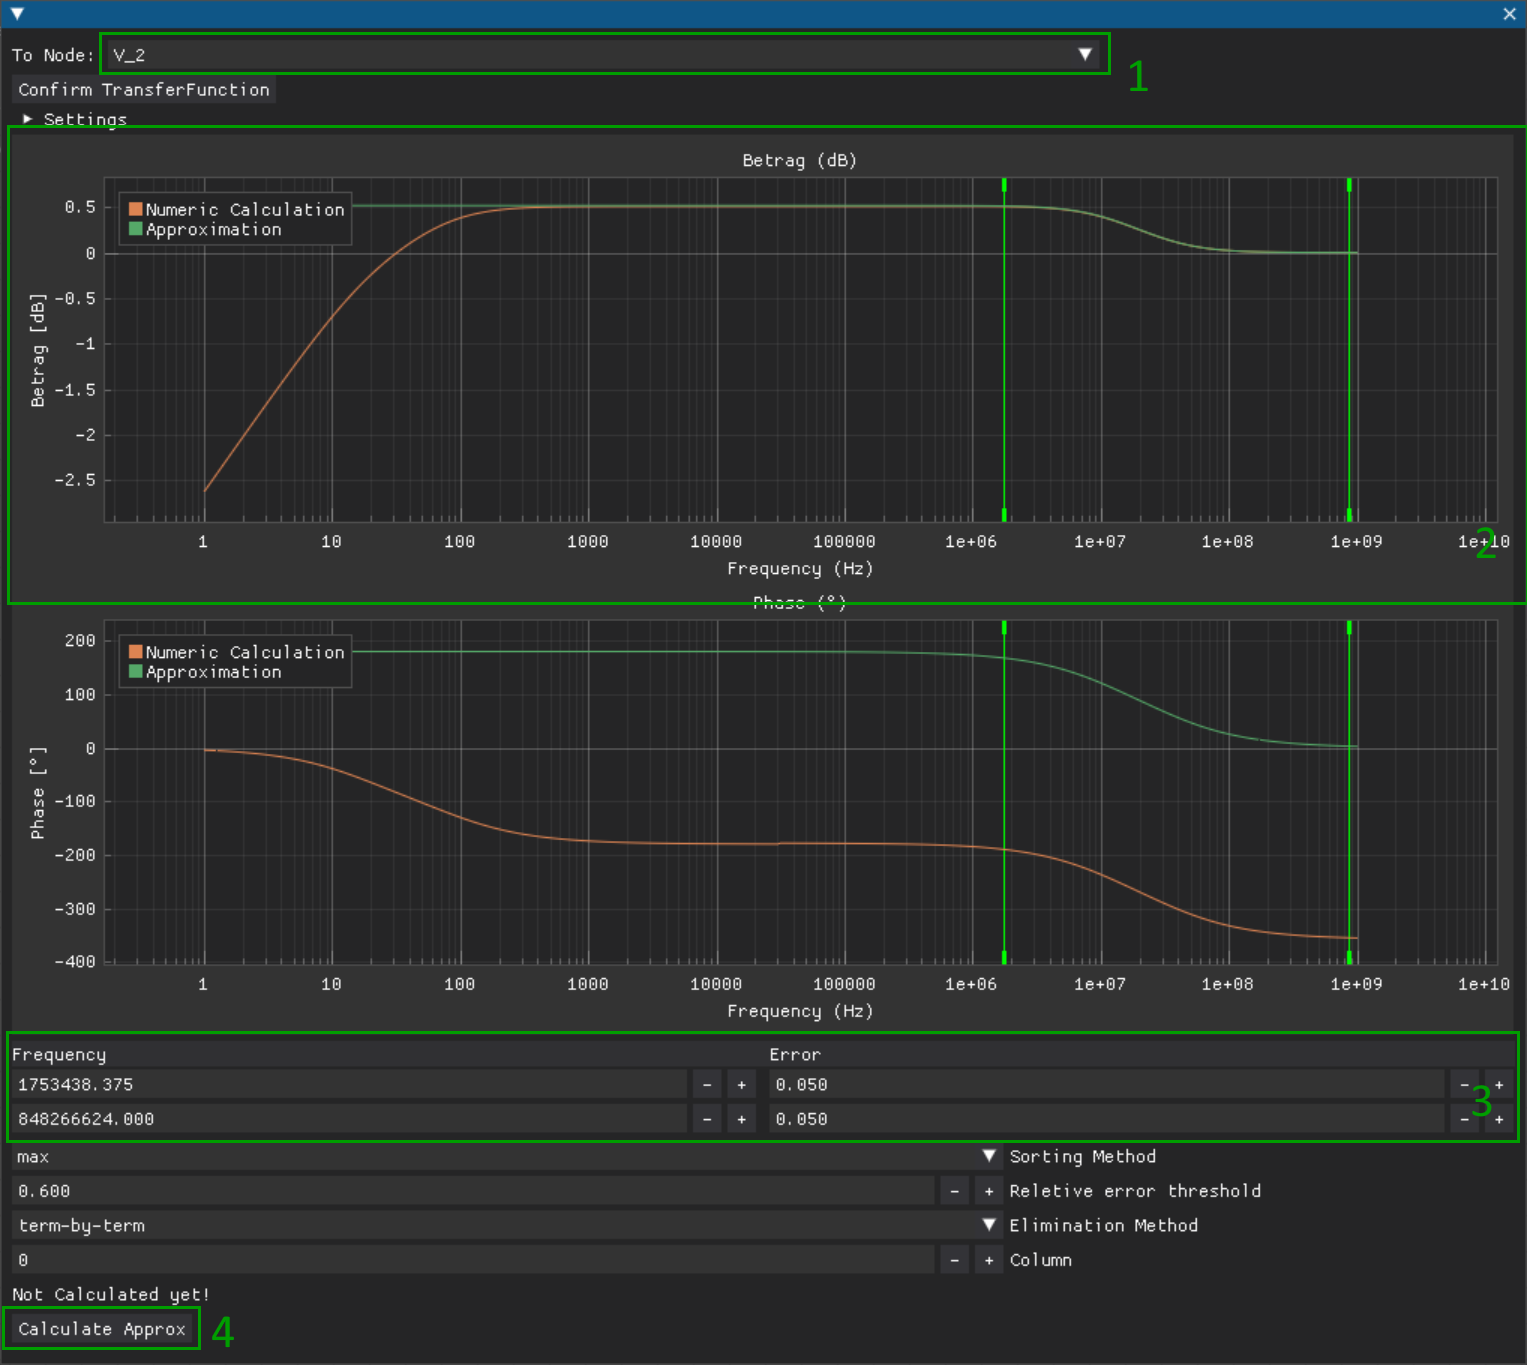
\includegraphics[width=0.8\textwidth]{bilder/window_approximate.png}
    \caption{Aufbau des Approximate Knotens}
    \label{fig:window_approximate}
\end{figure}

Folgende Einstellungen sind Relenvant.\\

\begin{itemize}
    \item \textbf{1. Bereich: } Im Ersten Bereich wird der Knoten ausgewählt über welchen Approximiert werden soll. Die Auswahl muss mit dem Knopf "Confirm Transferdunction" bestätigt werden.
    \item \textbf{2. Bereich:} Im Zweiten Bereich sieht mann ein BodePlot in welchen die Ausgewählte Übertragungsfunktion dargestellt wird. Mit Ctrl+Linksklick kann man das Mausposition ein Arbeitspunkt gewählt werden und mit Ctrl+ Rechtsklick wieder entfernt. Die Eingefügten Arbeitspunkte können mit dem Mauszeigen verschoben werden.
    \item \textbf{3. Bereich:} Hier ist eine Tabelle mit allen eingefügten Arbeitspunkten. Die Frequenzen können hier genau angepasst werden. Jedem Arbeitspunkt ist hier auch ein Fehler zugeordnet welcher auch Angepasst werden kann.
    \item \textbf{4. Bereich:} Durch diesen Button wird die Approximation berechnet. Auch diese wird dann im BodePlot dargestellt und kann mit der Originalfunktion vergleichen werden.
\end{itemize}


\subsection{Speichern und Laden von Analysen}
Der Aufgebaute Analysegraph kann über das Fensetermenu: "File"->"Save" gespeichert werden. Geladen wird über den Menupunkt "File" -> "Open". Mannche Knoten müssen nach dem laden in der richtigen reihenfolge ausgeführt werden, da nicht alle Ergebnisse gespeichert werden. Zum Beispiel werden die ausgerechneten Numerischen werte nicht gespeichert. 